\subsection{IMU Data Processing}
The IMU's data processing was implemented in the Programmable Software because it involves complex mathematics, and can be easily integrated with the rangefinder's data in the Xilinx Software Development Kit (SDK).

\subsubsection{Programmable Software}
The SPI communication in the SDK was customized and implemented by following example code provided with the SPIPS driver under the Xilinx SDK. The examples are located in the following folder: \path{C:\Xilinx\SDK\2016.2\data\embeddedsw\XilinxProcessorIPLib\drivers\spips_v3_0\examples\}.
\par
By following Xilinx's examples, the IMU's register settings were set and then the axis data was read from their respective registers. The axis data is signed and expressed in Two's Complement format\footnote{Two's Complement is a way of encoding signed numbers in binary where the most significant bit is used as a sign bit, with '1' signifying a negative number and '0' signifying a positive number. To convert a positive number to negative, all of the bits are inverted and then 1 is added to the resultant number \cite{2sComp}.} \cite{lsm9ds1}. The axis data is read into an array of unsigned 8-bit numbers. The data points are rearranged and then stored into an integer buffer for each axis. Combining the data in this manner would work if the $int$ data type were only 16 bits. However, the data type $int$ in the Xilinx SDK is 32 bits. For positive numbers this method is sufficient, but for negative numbers this process drops the sign bit. The sign bit is the most significant bit of the axes' 16-bit data, which gets lost when getting stored in a 32-bit integer. This problem was corrected by checking if the data stored in each axes' most significant word was greater than or equal to 80\textsubscript{16}. If greater than or equal to 80\textsubscript{16} then the sign bit must be '1', signifying a negative number. If necessary, the data was turned negative by subtracting FFFF\textsubscript{16}, or 65,535\textsubscript{10}, and adding 1.
\par
Before the complex math can be performed on the data, the header file $math.h$ must be included into the project. This is done by right clicking on the application project, choosing Properties $\rightarrow$ C/C++ Build $\rightarrow$ Settings $\rightarrow$ Tool Settings $\rightarrow$ ARM v7 gcc linker $\rightarrow$ Libraries, and then adding $m$ under the Libraries (-l) section, shown in Figure \ref{including_math}. In addition, $math.h$ still must be included by using $\#include$ in the project's source code file. This process allows the included $math.h$ header file to be linked into the project by the linker.

\begin{figure}[H]
	\centerline{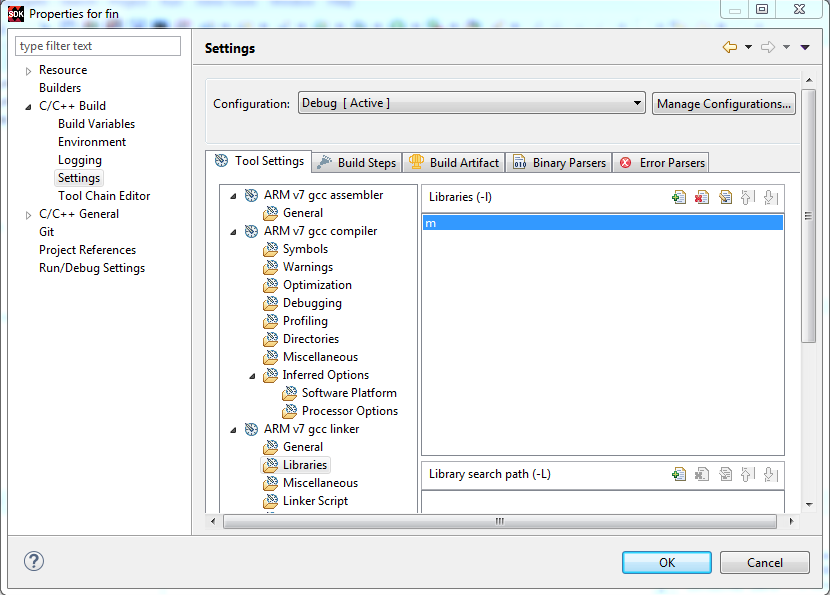
\includegraphics[width=1\textwidth]{including_math.png}}
	\caption{Linking $math.h$ into the Application Project in the SDK}
	\label{including_math}
\end{figure}

Once the magnetometer axis data was accurately stored in their corresponding buffers and $math.h$ properly linked, the data can begin its transformation. The data is expressed in terms of milligauss per bit, which is converted to a compass heading in degrees by using Equation \ref{GaussToDegrees}.

\begin{equation}
	\textrm{Compass Heading} = \arctan(\dfrac{y}{x})\times\dfrac{180}{\pi}
	\label{GaussToDegrees}
\end{equation}

To convert the compass heading to a rangefinder step offset, Equation \ref{CompassHeadingToStepOffset} was used.

\begin{equation}
	\textrm{Step Offset} = \dfrac{\textrm{Compass Heading}}{\dfrac{360^\circ}{1024\ steps}}
	\label{CompassHeadingToStepOffset}
\end{equation}

The resultant step offset is added to the rangefinder's step in order to account for the sensor suite's compass direction deviation from North. When the ZedBoard faces North the step offset equates to 0, so the rangefinder's data is not rotated. When the ZedBoard faces South the step offset equates to 512, which rotates the rangefinder data by $180^\circ$.






